% input from talk.tex or notes.tex.

\mode<presentation>
{
  \usetheme{default}
  \setbeamertemplate{navigation symbols}{}
  \setbeamertemplate{footline}[frame number]
  \setbeamertemplate{items}[circle]
  \usecolortheme{seahorse}
}

\usepackage[english]{babel}
\usepackage[utf8]{inputenc}
\usepackage{times}
\usepackage[T1]{fontenc}
\usepackage{url}

\newcommand\topstrut{\rule{0pt}{2.6ex}}
\newcommand\bottomstrut{\rule[-1.2ex]{0pt}{0pt}}
\newcommand\doublestrut{\rule[-1.2ex]{0pt}{3.6ex}}

\newcommand\gray[1]{\textcolor{gray}{#1}}
\newcommand\smallgray[1]{\textcolor{gray}{\small\it #1}}

\newcommand {\framedgraphic}[2] {
  \begin{frame}{#1}
    \begin{center}
      \includegraphics[width=\textwidth,height=0.89 \textheight,keepaspectratio]{#2}
    \end{center}
  \end{frame}
}
% A full-page graphic.
\newcommand {\graphic}[2] {
  \only<#1>{\centerline{\includegraphics[width=\textwidth,height=0.9\textheight,keepaspectratio]{#2}}}
}
% A graphic with a text caption.
\newcommand {\graphicT}[3] {
  \only<#1>{\centerline{\includegraphics[width=\textwidth,height=0.85\textheight,keepaspectratio]{#2}}
  \centerline{#3}}
}
% A box measuring one quarter the page.
\newcommand\boxQ[1] {
  \vbox to .42\textheight{\vfill\hbox to .5\textwidth{\hfill{#1}\hfill}\vfill}
}
% A quad box of graphics.
\newcommand\graphicQ[5] {
  \only<#1>{
    \centerline{\boxQ{\includegraphics[width=.5\textwidth,height=0.42\textheight,keepaspectratio]{#2}}
      \boxQ{\includegraphics[width=.5\textwidth,height=0.42\textheight,keepaspectratio]{#3}}}
    \centerline{\boxQ{\includegraphics[width=.5\textwidth,height=0.42\textheight,keepaspectratio]{#4}}
      \boxQ{\includegraphics[width=.5\textwidth,height=0.42\textheight,keepaspectratio]{#5}}}
  }}
% A quad box of graphics with a caption.
\newcommand\boxQT[2] {
  \boxQ{
    \vbox{
      \hbox{\includegraphics[width=.5\textwidth,height=0.36\textheight,keepaspectratio]{#1}}
      \hbox{#2}
    }
  }
}
% A split page, two images.
\newcommand\graphicD[3] {
  \only<#1>{
    \centerline{\includegraphics[width=.5\textwidth,height=0.9\textheight,keepaspectratio]{#2}
      \includegraphics[width=.5\textwidth,height=0.9\textheight,keepaspectratio]{#3}}
  }}
% A split page, two images, with subtitle
\newcommand\graphicDT[4] {
  \only<#1>{
    \centerline{\includegraphics[width=.5\textwidth,height=0.85\textheight,keepaspectratio]{#2}
      \includegraphics[width=.5\textwidth,height=0.85\textheight,keepaspectratio]{#3}}
    \centerline{#4}
  }}

\title{Business Models and Technology}
\subtitle{Change}

\author[Abrahamson] {Jeff Abrahamson} \institute{Jellybooks}

\date[Big-O Meetup]
{Audencia School of Management, 26 November 2014}

% If you wish to uncover everything in a step-wise fashion, uncomment
% the following command: 
%\beamerdefaultoverlayspecification{<+->}

\begin{document}

% \frame{\titlepage}

\begin{frame}
  \titlepage
\end{frame}
\note{
  \begin{itemize}
  \item Technology and business change, disruption
  \item ``Amazon didn't create a new business model''

  \item I'm CS
  \item Technology and business (not models)
  \item History for context
  \end{itemize}
}

\section{}
\subsection{}


\frame[plain]{
  \frametitle{Light}
  \graphic{1}{lamplighter-1.jpg}
  \graphic{2}{lamplighter-3.jpg}
}
\note{
  \begin{itemize}
  \item Lamp lighters out of work
  \item Different install/repair skills
  \item Fewer bulb changers
  \end{itemize}
}

\frame[plain]{
  \frametitle{Transport}
  \graphic{1}{horse_carriage-1.jpg}
  \graphic{2}{horse-bus-1.jpg}
  \graphic{3}{horse-bus-2.jpg}
  \graphic{4}{horses-american-cities.jpg}
  \graphic{5}{horse-street-cleaner.jpg}
}
\note{
  \begin{itemize}
  \item cars, buses, cities, infrastructure (cleaning)
  \end{itemize}
  end: street cleaner

  Looks hot out, cold drink? Plan in advance\dots
}

\frame[plain]{
  \frametitle{Refrigeration}
  \graphic{1}{ice-cutter.jpg}
  \graphic{2}{ice-cutters.jpg}
  \graphic{3}{ice-house-1.jpg}
  \graphic{4}{ice-house-2.jpg}
  \graphic{5}{ice-house-3.jpg}
  \graphic{6}{ice-house-florence.jpg}
  \graphic{7}{ice-house-chennai.jpg}
  \graphicT{8}{frederick-tudor.jpg}{Frederick Tudor, Ice King}
  \graphicT{9}{world-ice-trade_1856.png}{New England ice trade, 1856}
}
\note{
  \begin{itemize}
  \item Cut and store; scale up; luxury
  \item Indian - built 1842 - business collapsed in 1880 from steam process
  \item Frederick Tudor, Ice King of the World; American, established
    the ice trade; shipped ice to Caribbean, Europe, India from Boston
    (100 days); first ship went to Martinique
  \item Legal squabbles - ownership of ice sources
  \item Plant ice; steam process; refrigeration systems
  \end{itemize}
  end: NE ice trade
}

\frame[plain]{
  \frametitle{Music}
  \graphicQ{1}{vinyl.jpg}{nil.png}{nil.png}{nil.png}
  \graphicQ{2}{vinyl.jpg}{cd.jpg}{nil.png}{nil.png}
  \graphicQ{3}{vinyl.jpg}{cd.jpg}{itunes.png}{nil.png}
  \graphicQ{4}{vinyl.jpg}{cd.jpg}{itunes.png}{spotify.png}
}
\note{
  \begin{itemize}
  \item LP's -> CD's -> iTunes (electronic purchase) -> discovery services
  \item Similar for video: VHS -> DVD -> rental -> Netflix DVD -> Netflix streaming and discovery (e.g., youtube)
  \end{itemize}
  end: 
}

\frame[plain]{
  \frametitle{Photography}
  \graphic{1}{plate-camera}
  \graphicQ{2}{shackleton-1.jpg}{shackleton-2.jpg}{shackleton-3.jpg}{shackleton-4.jpg}
  \graphic{3}{land-camera.jpg}
  \graphicDT{4}{edwin-land-young.jpg}{edwin-land-old.jpg}{Edwin H. Land}
  \only<5>{
    \centerline{
      \boxQT{kodak_instamatic_100.jpg}{1970's}
      \boxQT{quicktake.jpg}{early 1990's}
    }
    \centerline{
      \boxQT{pas-camera.jpg}{2000's}
      \boxQT{EOS-300D.jpg}{2000's}
    }
  }
  \only<6>{
    \centerline{
      \boxQT{kodak_instamatic_100.jpg}{1970's}
      \boxQT{nikon-coolpix-800.jpg}{late 1990's}
    }
    \centerline{
      \boxQT{pas-camera.jpg}{2000's}
      \boxQT{EOS-300D.jpg}{2000's}
    }
  }
  \graphicD{7}{iphone.jpg}{EOS-5D.jpg}
}
\note{
  \begin{itemize}
  \item Ernest Shackleton's ship, the Endurance. Slowly
    crushed. Photographer Frank Hurley dove for plates.
  \item Edwin Land, 1947 camera. First instant camera. Niche market compared to roll film.
  \item MIT story, Columbia lab, 9th floor (U.S.) window, first
    inexpensive polarizing film, led to founding Polaroid
    Corporation.
  \item Evolution of technology (quicktake only Si Valley, really)
  \item Now two main markets left, and photographers get paid less, due also to internet stock photography
  \end{itemize}
  end: 
}


\frame[plain]{
  \frametitle{Cleaning}
  \graphicQ{1}{man-baby-cleaning.jpg}{man-vacuuming.jpg}{nil.png}{nil.png}
  \graphicQ{2}{man-baby-cleaning.jpg}{man-vacuuming.jpg}{man-vacuuming-2.jpg}{nil.png}
  \graphicQ{3}{man-baby-cleaning.jpg}{man-vacuuming.jpg}{roomba.jpg}{nil.png}
  \graphicQ{4}{man-baby-cleaning.jpg}{man-vacuuming.jpg}{roomba.jpg}{man-cleaning.jpg}
}
\note{
  \begin{itemize}
  \item Cleaning takes time
  \item Or hire someone
  \item Or a machine does it
  \item Maybe a bit left to do by hand
  \end{itemize}
  end: guy with bucket
}


\frame[plain]{
  \frametitle{Real Estate}
  \graphic{1}{estate-agent-1.jpg}
  \graphic{2}{estate-agent-leboncoin.png}
  \graphic{3}{estate-agent-redfin.png}
}
\note{
  \begin{itemize}
  \item Anglosaxon world: agents
  \item France: p2p
  \item Increasingly: internet
  \item Redfin: hybrid
  \end{itemize}
  end: redfin
}

\frame[plain]{
  \frametitle{Personal Transport}
  \graphic{1}{london-taxi.jpg}
  \graphic{2}{I-80_Eastshore_Freeway.jpg}
  \graphic{3}{uber-1.png}
  \graphic{4}{hailo.jpg}
  \graphic{5}{paris-taxi-strike.jpg}
  \graphic{6}{uber-2.png}
  \graphic{7}{blablacar.jpg}
  \graphic{8}{google-car.jpg}
}
\note{
  \begin{itemize}
  \item UK, US
  \item Cities now
  \item London response (adopt new business techniques).  French response (old business techniques).
  \item One rebranding effort
  \item Outside cities, ride sharing (more efficient than decades past)
  \item Self-driving cars (taxis, car dealers (ownership), data, urban
    infrastructure (parking, safety margins); public health; Cars-as-a-Service)
  \end{itemize}
  end: Google car

  transition: want to make a phone call, 30 years ago became possible
}

\frame[plain]{
  \frametitle{Mobile communication}
  \graphic{1}{first-car-phone.jpg}
  \graphic{2}{nokia.jpg}
  \graphic{3}{iphone-6.png}
  \graphic{4}{N5-4G.png}
  \graphic{5}{4G.png}
  \graphic{6}{wifi.png}
  \graphicT{7}{dozendp_1.jpg}{Gongkai, \$12}
  \graphicQ{8}{loon-2.png}{loon-1.jpg}{loon-3.png}{loon-4.jpg}
  \graphic{9}{facebook-drone-1.jpg}
}
\note{
  \begin{itemize}
  \item Initially, filling non-existent need
  \item Disruption 1 (and running out of phone numbers)
  \item Disruption 2 (iPhone 29 Jun 2007)
  \item iphone (30-50m sold per quarter); android (50-90m sold per quarter)
  \item Instagram (10/2010 release; 4/2012 1e8 active users  and fb purchase at \$1e9)
  \item Phone now tcp/ip device
  \item Democratization, ubiquitous networks; non-wiring the third world
  \end{itemize}
  end: fb drone

  transition: what pays for this?
}

\frame[plain]{
  \frametitle{Advertising}
  \graphic{1}{newspaper-1.jpg}
  \graphic{2}{hearst-castle-pool.jpg}
  \graphicQ{3}{search.jpg}{gmaps.png}{news.jpg}{facebook-share.jpg}
  \graphicQ{4}{wapping-1.jpg}{wapping-2.jpg}{wapping-3.jpg}{wapping-4.jpg}
}
\note{
  \begin{itemize}
  \item Newspapers sell copies, but mostly sell advertising. News is the waste product.
  \item Hearst Castle, San Simeon; William Randolph Hearst
  \item Now waste product is search, maps, news, social, email
  \item Meanwhile, newspapers ripe for disruption; 24 Jan 1986 typesetters strike; Musée de l'Imprimerie
  \end{itemize}
  end: 
}

\frame[plain]{
  \frametitle{Translation}
  \graphic{1}{translate.jpg}
  \graphic{2}{the-turk.jpg}
}
\note{
  \begin{itemize}
  \item Most translation is now machine
  \item Humans internet delivery (non-local clients), TZ shift, lower wages
  \item Democratization: individuals, web browsers, translate.google.com
  \item Mechanical Turk (\$1/hr), captchas
  \item (The Turk, 1770 ff, Wolgang von Kempelen)
  \end{itemize}
  end: The Turk
}

\frame[plain]{
  \frametitle{Books}
  \graphic{1}{books.jpg}
  \only<2>{
    \centerline{\boxQ{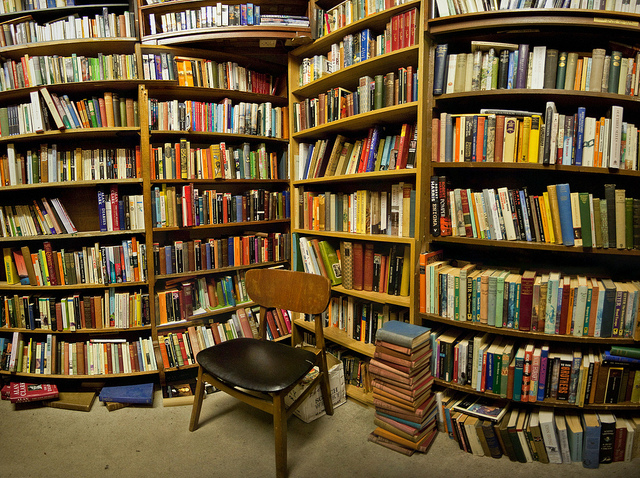
\includegraphics[width=.5\textwidth,height=0.85\textheight,keepaspectratio]{books.jpg}}
      \boxQ{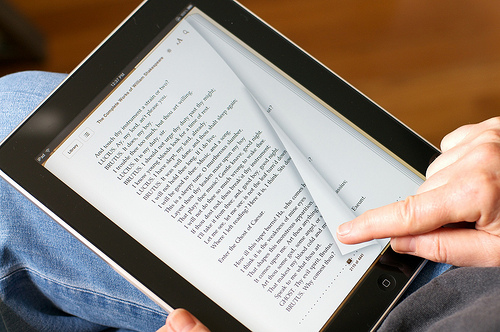
\includegraphics[width=.5\textwidth,height=0.85\textheight,keepaspectratio]{ebook.jpg}}}
  }
}
\note{
  \begin{itemize}
  \item Self-publishing used to be unrespectable, now majority
  \item Long tail effect (below cost of advance, publisher's efforts)
  \item Niche audiences possible
  \item Blogs, wikipedia (encyclopedias killed by PC's)
  \item At high end, more profit (e.g., J.~K.~Rowlings ebook versions)
  \item Kindle Scout = crowd sourced
  \item Not clear yet how this will affect book publishing and book-related businesses
  \end{itemize}
  end: 
}

\frame[plain]{
  \frametitle{Tech Startups}
  \graphic{1}{google-data-center-1.jpg}
  \graphic{2}{google-data-center-2.jpg}
  \graphic{3}{zero-to-one.jpg}
%  \graphic{4}{}
%  \graphic{5}{}
}
\note{
  \begin{itemize}
  \item AWS, Google etc. means low startup costs
  \item Most services available free or for rent (cheap)
  \item Example: Whatsapp, 600m users, 50 people, \$19b
  \item Peter Thiel (Paypal, Palantir) - good ideas should seem like bad ideas to most people
  \end{itemize}
  end: Zero to One
}

\frame[plain]{
  \frametitle{Risk}
  \graphic{1}{trading-floor-1.jpg}
  \graphic{2}{trading-floor-jeff.jpg}
%  \graphic{3}{}
%  \graphic{4}{}
%  \graphic{5}{}
}
\note{
  \begin{itemize}
  \item Risk is derivative of something (often price) with respect to
    something (high dimensional manifold (hopefully))
  \item 1e6 computer hours per day [press]
  \item Pricing accuracy determines profit expectations
  \item Story about interactive counterparty risk (start with RT and ON risk)
  \end{itemize}
  end: 
}

\frame[plain]{
  \frametitle{Education,}
  \graphic{1}{mooc.png}
  \graphic{2}{ring.jpg}
}
\note{
  Problems:
  \begin{itemize}
  \item Free (for now)
  \item Identifying people
  \item Preventing cheats
  \item Recognition of diplomas
  \end{itemize}
  Maybe one or two universities per major language.
  
  end: ring
}


\begin{frame}
  \frametitle{Questions}

  \vbox to .9\textheight{\vfill\hbox to .9\textwidth{\hfill{
\includegraphics[height=.7\textheight,keepaspectratio]{question-mark.jpg}}\hfill}\vfill}
\end{frame}

\end{document}
